\section{Results: the zoom audit}
\label{sec:results}

\newcommand{\maybefig}[1]{\IfFileExists{fig/#1.pdf}{\includegraphics[width=\linewidth]{fig/#1.pdf}}{\fbox{\small figure #1 pending}}}

\begin{figure*}[t]
  \centering
  \IfFileExists{fig/teaser.pdf}{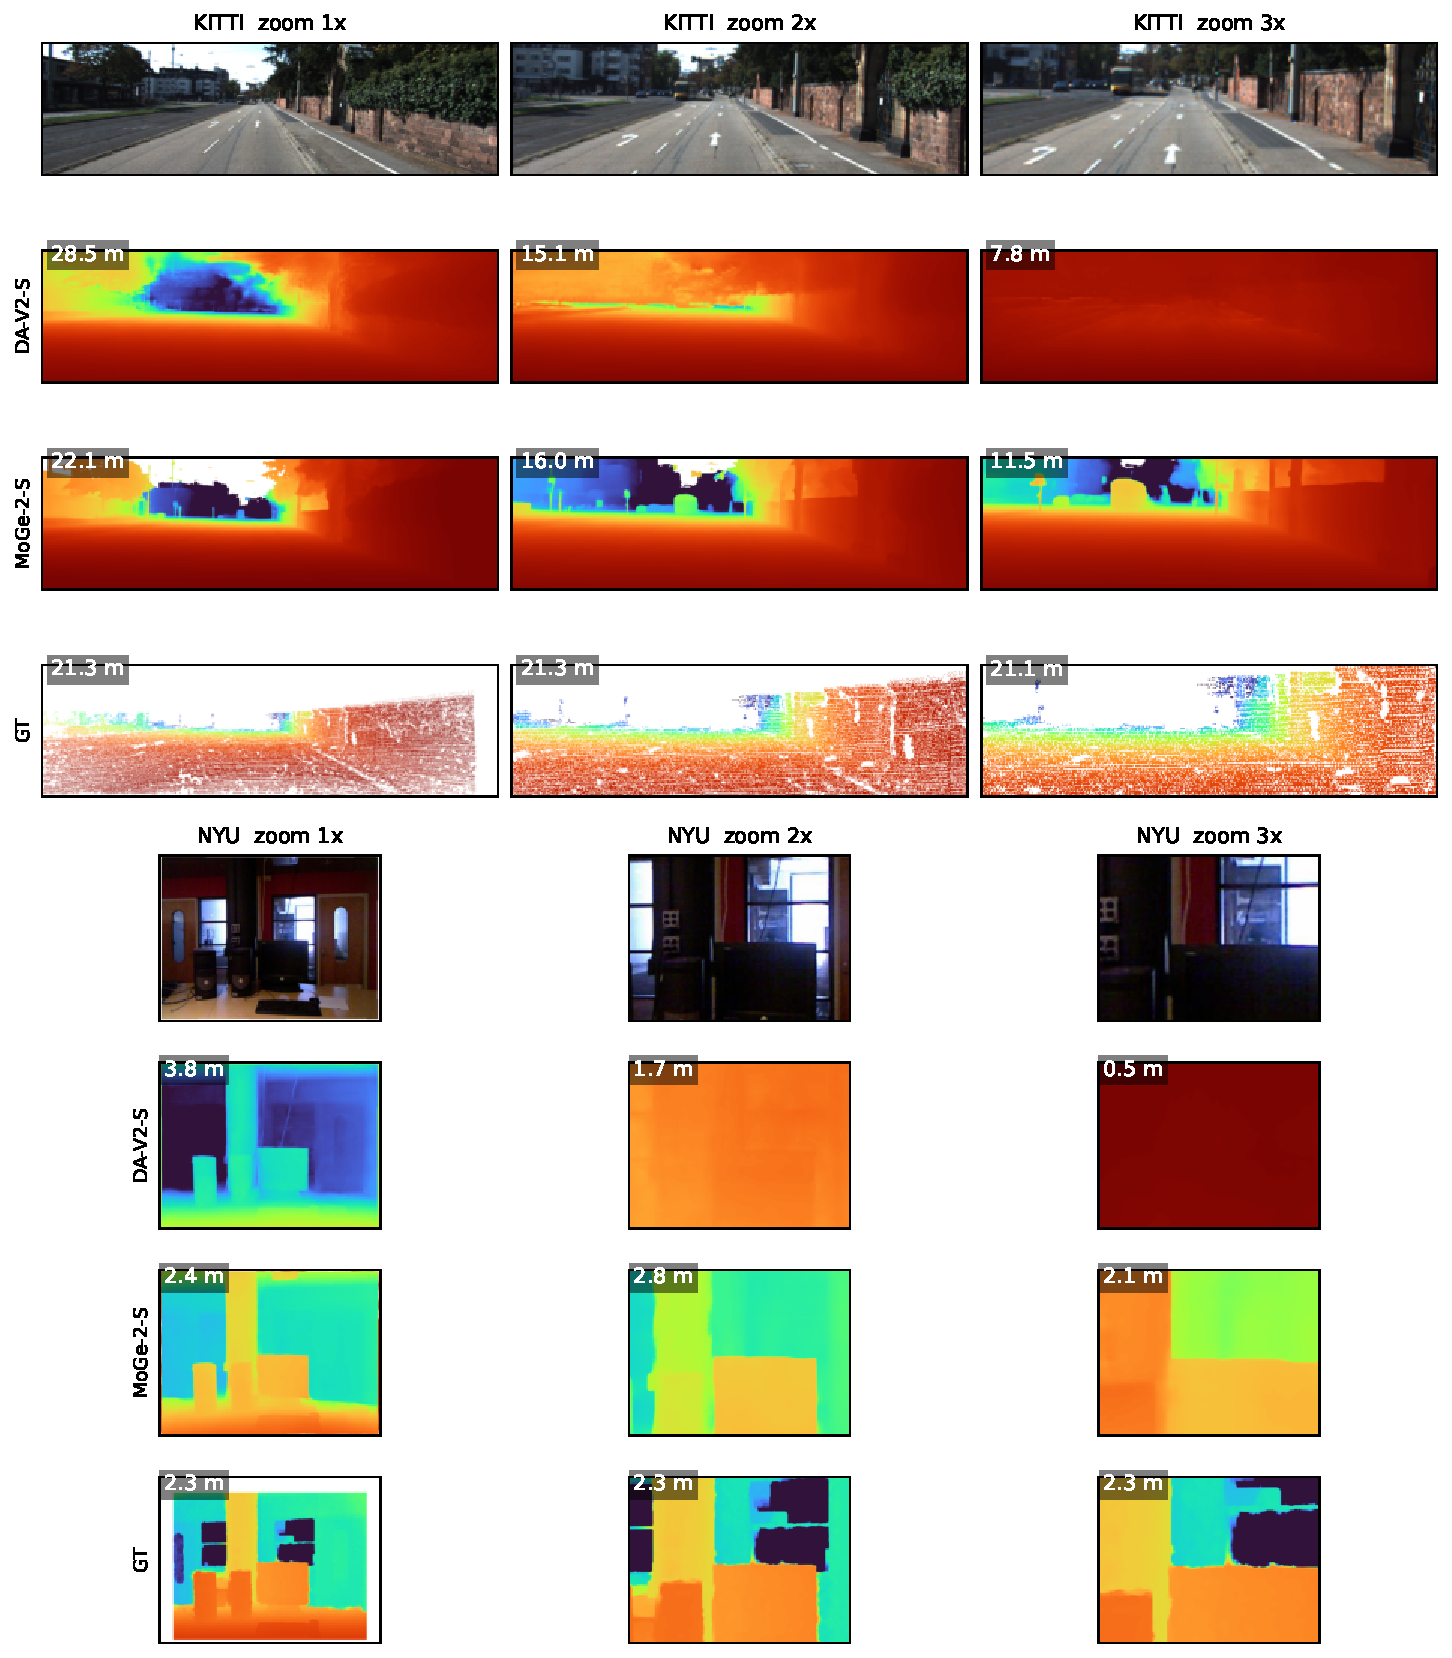
\includegraphics[width=\linewidth]{fig/teaser.pdf}}{\fbox{teaser pending}}
  \caption{A KITTI image at $1\times$, $2\times$ and $3\times$ digital zoom. All depth panels share one
  colour scale (metres); the number is the median depth of the pixels inside the $3\times$ crop, i.e. the
  same physical points in every column. Depth Anything V2 moves the scene closer as we zoom in (28.5\,m to
  7.8\,m); MoGe-2, which predicts its camera, moves it less; the LiDAR ground truth does not move.
  An NYUv2 example is in the supplement.}
  \label{fig:teaser}
\end{figure*}

\begin{table*}[t]\centering\small
\caption{Zoom audit, pooled over KITTI, NYUv2, DIODE-indoor and DIODE-outdoor (\nImages{} images per model, \nScenes{} scenes). $\alpha$: depth exponent (ideal 0; apparent size only: 1), median over images with a 95\% interval from a scene-level bootstrap. $\beta$: focal exponent (ideal 1). $\alpha+\beta$: median per image (1 = lateral sizes kept, \cref{sec:law}). Blur: depth change under the blur control. AbsRel at $1\times$ on the full image, and at $3\times$ on the crop for the unzoomed prediction (``same px'') and the zoomed one.}
\label{tab:audit}
\setlength{\tabcolsep}{4pt}
\begin{tabular}{llccccccc}\toprule
& & & & & & \multicolumn{3}{c}{AbsRel} \\ \cmidrule(lr){7-9}
Model & Group & $\alpha$ & $\beta$ & $\alpha+\beta$ & Blur & $1\times$ & $3\times$ same px & $3\times$ zoomed \\ \midrule
DA-V2-S & pixels only & 0.95 [0.83, 1.12] & -- & -- & 1.3\% & 0.317 & -- & 0.652 \\
DA-V2-B & pixels only & 0.85 [0.76, 0.94] & -- & -- & 0.8\% & 0.313 & -- & 0.599 \\
ZoeDepth & pixels only & 0.61 [0.52, 0.75] & -- & -- & 0.7\% & 0.310 & -- & 0.539 \\
Depth Pro & predicts camera & 0.31 [0.20, 0.40] & 0.65 & 0.97 & 2.8\% & 0.310 & 0.293 & 0.459 \\
MoGe-2-S & predicts camera & 0.36 [0.30, 0.40] & 0.56 & 0.95 & 3.1\% & 0.274 & -- & 0.465 \\
UniDepthV2-S & predicts camera & 0.34 [0.23, 0.50] & 0.45 & 0.87 & 4.1\% & 0.824 & -- & 0.792 \\
Metric3D v2-S & takes camera (true K) & -0.07 [-0.11, -0.05] & -- & -- & 1.6\% & 0.142 & -- & 0.358 \\
Metric3D v2-S (stale K) & takes camera (stale K) & 0.93 [0.89, 0.95] & -- & -- & 1.6\% & 0.142 & -- & 0.628 \\
\bottomrule\end{tabular}\end{table*}


\paragraph{No image-only model respects the zoom (H1).}
\Cref{tab:audit} and \cref{fig:curves} summarise \nImages{} images per model. The pixels-only models
shrink depth almost like $1/s$: $\alpha=\DavTwoSAlpha$ [\DavTwoSAlphaLo, \DavTwoSAlphaHi] for
DA-V2-S, \DavTwoBAlpha{} for DA-V2-B and \ZoedepthAlpha{} for ZoeDepth. A $3\times$ zoom thus moves a
scene to about \DavTwoSRatioThree{} of its predicted distance. Models that predict their camera do
better but are far from equivariant ($\alpha$ between \DepthproAlpha{} and \MogeTwoSAlpha), and their
focal estimate grows by only \UnidepthTwoSFocalThree--\DepthproFocalThree{} at $3\times$ instead of
$3$. Metric3D with the correct $K'$ is close to the law ($\alpha=\MetricThreedSAlpha$, a slight
over-correction), and with the stale $K$ its exponent is $\alpha=\MetricThreedSStaleKAlpha$, larger by
\staleDiff{} per image as derived in \cref{sec:law}. The zoom costs accuracy accordingly: on the
same pixels, the AbsRel of DA-V2-S grows from \DavTwoSBaseThree{} unzoomed to \DavTwoSAbsrelThree{}
at $3\times$. Intervals in \cref{tab:audit} resample whole scenes (\nScenes{} in total); the
image-level intervals are much narrower and would overstate certainty.

\begin{figure}[t]
  \centering
  \maybefig{fig2_depth_and_focal_vs_zoom}
  \caption{Depth (left) and predicted focal (right) of the same pixels as a function of the zoom factor,
  median over images. Dashed: the law; dotted: apparent size only.}
  \label{fig:curves}
\end{figure}

\paragraph{The failure follows apparent size (H2).}
\Cref{fig:abplane} places each camera-predicting model in the $(\beta,\alpha)$ plane. Depth Pro lies on
the line $\alpha+\beta=1$ (median \DepthproAlphaPlusBeta{} per image), MoGe-2 close to it
(\MogeTwoSAlphaPlusBeta) and UniDepthV2 below it (\UnidepthTwoSAlphaPlusBeta). On this line a model keeps
the lateral size of what it sees but not its depth, which is exactly the interpretation the
zoom--squash ambiguity makes available: the zoomed image is consistent with a compressed scene in which
every object keeps its width. A softer reading of the ambiguity, that scenes with a larger depth range
would be easier, is not supported: the within-dataset rank correlation between $\alpha$ and the
inter-quartile range of log depth is \DepthproSpreadRho{} for Depth Pro and \MogeTwoSSpreadRho{} for
MoGe-2. The ambiguity explains the direction of the failure, not which images escape it.

\begin{figure}[t]
  \centering
  \IfFileExists{fig/fig3_alpha_beta_plane.pdf}{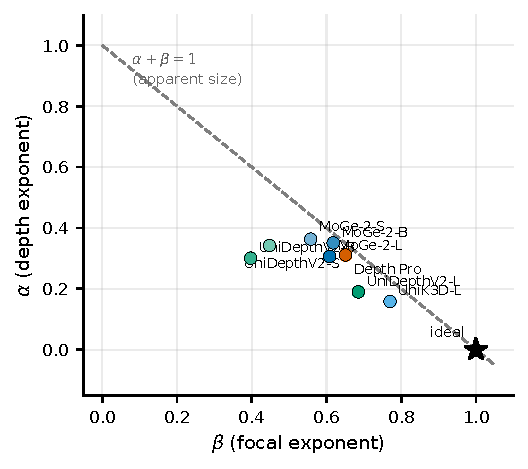
\includegraphics[width=0.78\linewidth]{fig/fig3_alpha_beta_plane.pdf}}{\fbox{pending}}
  \caption{Camera-predicting models in the $(\beta,\alpha)$ plane. Dashed: $\alpha+\beta=1$, where
  lateral sizes are preserved (apparent-size reasoning). The ideal model is at $(1,0)$.}
  \label{fig:abplane}
\end{figure}

\paragraph{It is the camera, not the pixels.}
The blur control, which loses as much detail as a $2\times$ zoom without changing the field of view,
moves depth by only \DavTwoSBlur\% for DA-V2-S and at most \UnidepthTwoSBlur\% for any model in
\cref{tab:audit}. \Cref{tab:controls} separates the two effects of a digital zoom directly: an
\emph{optical} $2\times$ zoom with real detail changes the depth of DA-V2-S by a factor of
\DavTwoSOptical, the same zoom done digitally by \DavTwoSDigitalLr, while bilinear resampling and JPEG
compression change it by \DavTwoSBilinear{} and \DavTwoSJpeg.
% TODO(results): one sentence on optical vs digital once audit-d is in.

\begin{table}[t]\centering\small
\caption{Confounder controls: median depth ratio on the same pixels (1 = unchanged). Optical: real-detail $2\times$ zoom of a half-resolution camera; digital: the same zoom by crop and up-sampling; bilinear: the $2\times$ digital zoom with bilinear resampling; JPEG: quality 75, no zoom.}\label{tab:controls}
\setlength{\tabcolsep}{4pt}
\begin{tabular}{lcccc}\toprule
Model & optical $2\times$ & digital $2\times$ & bilinear $2\times$ & JPEG \\ \midrule
DA-V2-S & -- & -- & -- & -- \\
Depth Pro & -- & -- & -- & -- \\
MoGe-2-S & -- & -- & -- & -- \\
Metric3D v2-S & -- & -- & -- & -- \\
\bottomrule\end{tabular}\end{table}


\paragraph{Bigger and newer models.}
\Cref{tab:ladder} extends the audit to larger variants and to Depth Anything~3, UniK3D and VGGT
(100 images per set; 50 for the DA3 and VGGT runs). On the \nLadderShared{} images that every model saw,
size helps the pixels-only family but does not remove the effect: $\alpha$ falls from \DavTwoSAlphaShared{}
(DA-V2-S) to \DavTwoBAlphaShared{} (B) and \DavTwoLAlphaShared{} (L), so the large model still returns less
than half the depth at $3\times$. MoGe-2 is flat across sizes (\MogeTwoSAlphaShared, \MogeTwoBAlphaShared,
\MogeTwoLAlphaShared), with a focal exponent stuck near \MogeTwoLBetaShared. UniDepthV2 improves with size
(\UnidepthTwoSAlphaShared{} to \UnidepthTwoLAlphaShared, $\beta$ from \UnidepthTwoSBetaShared{} to
\UnidepthTwoLBetaShared), and UniK3D-L, the newest camera-predicting model, comes closest
($\alpha=\UnikThreedLAlphaShared$, $\beta=\UnikThreedLBetaShared$). None reaches the level of a model that
is given the correct camera (Metric3D v2, $\alpha=\MetricThreedSAlphaShared$). Scale and newer camera heads
narrow the gap; they do not close it.
% TODO(results): add DA3 and VGGT once audit-c2 is in.

\begin{table}[t]\centering\small
\caption{Model ladder: larger variants and newer families. DA3-L and VGGT normalise depth per scene, so only $\beta$ is defined for them.}\label{tab:ladder}
\setlength{\tabcolsep}{3pt}
\begin{tabular}{llccc}\toprule
Model & Group & $\alpha$ & $\beta$ & images \\ \midrule
DA-V2-S & pixels only & 0.95 & -- & 800 \\
DA-V2-B & pixels only & 0.85 & -- & 800 \\
ZoeDepth & pixels only & 0.61 & -- & 800 \\
Depth Pro & predicts camera & 0.31 & 0.65 & 800 \\
MoGe-2-S & predicts camera & 0.36 & 0.56 & 800 \\
UniDepthV2-S & predicts camera & 0.34 & 0.45 & 800 \\
Metric3D v2-S & takes camera (true K) & -0.07 & -- & 800 \\
\bottomrule\end{tabular}\end{table}


\paragraph{Crop position and principal point.}
Zooming into the four image quadrants instead of the centre leaves $\alpha$ of the same order (supplement).
For a $2\times$ crop of an image quadrant the law moves the principal point by half the image width.
Both models that predict it ignore the move: the error of MoGe-2 (\MogeTwoSPpQuadTwo{} of the width) and of
UniDepthV2 (\UnidepthTwoSPpQuadTwo) equals that of always answering the image centre
(\MogeTwoSPpGuessTwo). Off-centre crops, which phone and detection crops usually are, are outside what
their camera models express.

\paragraph{When does the label-free score predict error?}
Across the \proxyPairs{} model--dataset pairs, $|\alpha|$ rank-correlates with AbsRel at $3\times$
(Spearman \proxyRhoThree{}, 95\% interval [\proxyRhoThreeLo, \proxyRhoThreeHi]) and within KITTI, NYUv2
and DIODE-indoor (\ProxyKitti, \ProxyNyu, \ProxyDiodeIn), but not within DIODE-outdoor
(\ProxyDiodeOut), where errors are dominated by a heavy tail of UniDepthV2. It does not predict
accuracy on unzoomed images (\proxyRhoOne). Part of the association is mechanical, since a shrinking
depth is also a growing error, so we read it narrowly: without labels, the audit tells which model will
degrade most under zoom, not which model is more accurate.

\paragraph{A training-free fix when the zoom is known.}
Phones record a digital zoom ratio, and apps know their own crops. Since $\alpha$ needs no labels, a
user can measure it on their own photos and multiply the depth of zoomed images by $s^{\hat\alpha}$.
We evaluate this cross-fitted: $\hat\alpha$ is measured on half of a dataset's images and the
correction scored on the other half. For DA-V2-S at $3\times$ the AbsRel goes from \DavTwoSFixZoomed{}
to \DavTwoSFixAbsrel{}, against \DavTwoSFixTarget{} for the unzoomed prediction on the same pixels.
A single global factor cannot undo everything: the zoomed prediction is also distorted in shape
(\cref{sec:audit}), which the remaining gap reflects.
% TODO(results): check once audit-a2 (fix columns) is in.
